\documentclass[tikz,border=10pt]{standalone}
\begin{document}
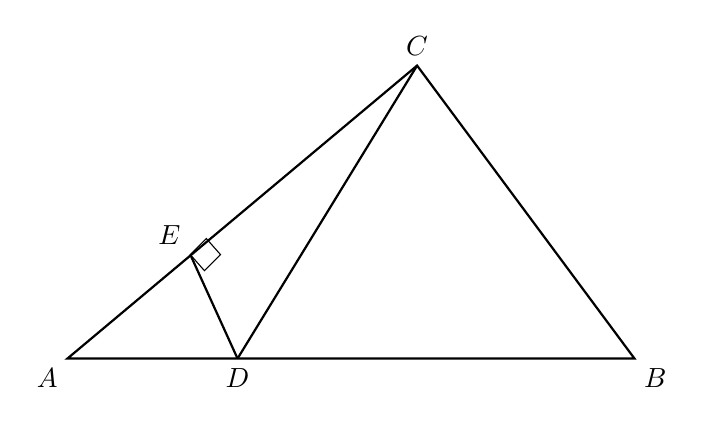
\begin{tikzpicture}[scale=1.2]
\coordinate (A) at (0,0);
\coordinate (B) at (6,0);
\coordinate (C) at (3.7,3.1);
\coordinate (D) at (1.8,0);
\coordinate (E) at (1.3,1.1);
\draw[thick] (A) -- (B) -- (C) -- cycle;
\draw[thick] (C) -- (D);
\draw[thick] (D) -- (E);
\draw (1.45,0.93) -- (1.62,1.10) -- (1.47,1.27) -- (1.30,1.10) -- cycle;
\node[below left] at (A) {$A$};
\node[below right] at (B) {$B$};
\node[above] at (C) {$C$};
\node[below] at (D) {$D$};
\node[above left] at (E) {$E$};
\end{tikzpicture}
\end{document}
